\chapter{The big picture}

\section{What you built, in three sentences}

You built a program that shrinks a grayscale picture to a small fraction of its size by throwing away the details a human eye barely notices, and a second program that rebuilds the picture from the small file.
It does this with exactly the recipe of the JPEG standard: cut the picture into $8\times 8$ tiles, re-express each tile as a mix of simple wave patterns (the \emph{DCT}), round the mix coarsely (\emph{quantization}, the only step that loses information), and then write the rounded numbers down in a compact shorthand (\emph{zig-zag, run-length, Huffman}).
You then measured how small the files get, how much quality is lost, how accurate the arithmetic is, and where the running time goes.

\begin{plain}
Compression is possible because pictures are \emph{predictable}: neighbouring pixels look alike, and our eyes are forgiving about fine detail.
The whole codec is a machine for (1) turning ``predictable'' into ``lots of zeros'' and (2) writing lots of zeros very cheaply.
\end{plain}

\section{The pipeline}

\begin{figure}[h]
\centering
\begin{tikzpicture}[node distance=0.55cm and 0.45cm,
  stage/.style={draw=accent,fill=plainbg,rounded corners=2pt,minimum height=0.95cm,minimum width=1.9cm,align=center,font=\footnotesize},
  lossy/.style={draw=warnfg,fill=warnbg,rounded corners=2pt,minimum height=0.95cm,minimum width=1.9cm,align=center,font=\footnotesize},
  arr/.style={-{Stealth[length=2mm]},thick}]
\node[stage] (a) {pixels\\$w\times h$};
\node[stage,right=of a] (b) {cut into\\$8\times 8$ tiles\\{\scriptsize $-128$}};
\node[stage,right=of b] (c) {DCT\\{\scriptsize per tile}};
\node[lossy,right=of c] (d) {quantize\\{\scriptsize \textbf{lossy}}};
\node[stage,below=0.9cm of d] (e) {zig-zag\\order};
\node[stage,left=of e] (f) {DC diff +\\run-length};
\node[stage,left=of f] (g) {Huffman\\code};
\node[stage,left=of g] (h) {\file{.jlc}\\file};
\draw[arr] (a)--(b); \draw[arr] (b)--(c); \draw[arr] (c)--(d); \draw[arr] (d)--(e);
\draw[arr] (e)--(f); \draw[arr] (f)--(g); \draw[arr] (g)--(h);
\node[font=\small\bfseries,color=accent,above=0.15cm of c] {ENCODER};
\end{tikzpicture}
\caption{The encoder. The decoder is the same chain run backwards (Huffman decode $\to$ de-zig-zag $\to$ multiply by the step sizes $\to$ inverse DCT $\to$ add 128 and round). Only the orange box destroys information.}
\end{figure}

\section{What the quality slider does to a picture}

\begin{figure}[h]
\centering
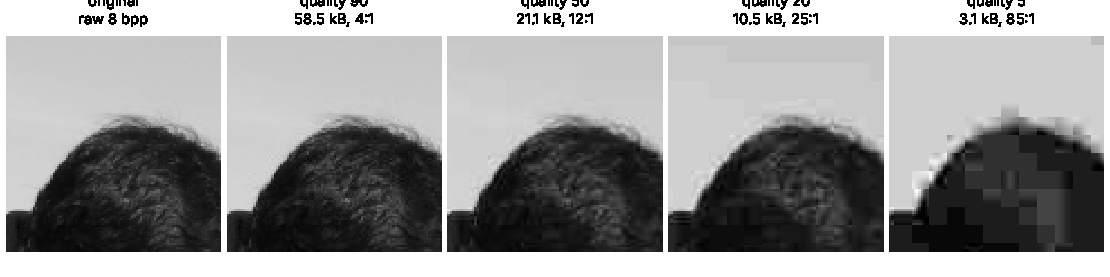
\includegraphics[width=\textwidth]{figures/quality_gallery.pdf}
\caption{A $96\times96$ crop of the test photograph (the ``cameraman'') through the codec. File sizes are for the whole $512\times512$ image. At quality~5 you can see the $8\times8$ tiles: that ``blocking'' is the signature of JPEG-style compression.}
\end{figure}

\section{Where everything lives}

\begin{longtable}{@{}p{4.6cm}p{10.4cm}@{}}
\toprule
\textbf{File} & \textbf{What it does}\\ \midrule\endhead
\file{include/jlc/*.hpp} & Public headers, each with a comment block explaining the idea.\\
\file{src/dct.cpp} & The $8\times8$ DCT / inverse DCT (matrix form) plus a slow textbook version used only by tests.\\
\file{src/quant.cpp}, \file{quant.hpp} & Step-size table, the quality scaling rule, and the rounding rule.\\
\file{src/zigzag.cpp} & Builds the zig-zag scan order.\\
\file{src/rle.cpp} & Turns a block into tokens: DC difference, (run, size) pairs, ZRL, EOB.\\
\file{src/huffman.cpp} & Builds Huffman code lengths, canonical codes, table (de)serialization, decoding.\\
\file{include/jlc/bitio.hpp} & Writing and reading individual bits.\\
\file{src/codec.cpp} & \code{encode()} and \code{decode()}: the whole pipeline, with per-stage timers.\\
\file{src/metrics.cpp} & MSE, PSNR, maximum error.\\
\file{apps/jlc\_cli.cpp} & Command line tool \code{jlc} (encode, decode, eval, sweep).\\
\file{apps/jlc\_bench.cpp} & Benchmark: median per-stage times, CSV output.\\
\file{tests/test\_main.cpp} & 28 test groups, 30\,000+ checks, no external framework.\\
\file{python/jlc\_ref.py} & Independent NumPy re-implementation that reads and writes the same file format.\\
\file{python/crosscheck.py} & Proves C++ and NumPy produce byte-identical files.\\
\file{python/rd\_sweep.py} & Rate--distortion sweep (also against libjpeg).\\
\file{python/numerics\_study.py} & Rounding, range, and precision experiments.\\
\file{slurm/*.sbatch} & Job scripts for bwUniCluster.\\ \bottomrule
\end{longtable}

\section{What this project is, and what it is not}

Being precise about scope makes you \emph{more} credible in an interview, so here it is plainly.

\begin{itemize}
\item \textbf{It is} a complete, working, tested lossy codec for 8-bit grayscale images, using the same algorithmic ingredients as baseline JPEG, validated against libjpeg (same distortion at the same quality, file sizes within about 1\%).
\item \textbf{It is not} a drop-in JPEG file reader/writer. The file format (``JLC1'') is our own: no JFIF headers, no marker bytes, one set of Huffman tables per image, no byte stuffing.
\item \textbf{It does not} handle colour. Real JPEG converts RGB to YCbCr and subsamples the colour channels; this project is luminance only. Chapter~\ref{ch:qa} has the answer to ``how would you add colour?''.
\item \textbf{It is single-threaded.} Parallelism (OpenMP over tiles, SIMD across tiles) is discussed as the next step in Chapter~\ref{ch:perf}, not claimed as done.
\end{itemize}

\begin{warn}[Honesty rule for the interview]
Say ``JPEG-\emph{like}'' exactly as the resume does. Anyone who knows JPEG will respect a precise list of what you implemented and what you deliberately left out far more than a vague claim to have ``built JPEG''.
\end{warn}

\section{How to use this guide}

\begin{enumerate}
\item Read Chapters~2--7 once, slowly, with the code open next to you. They explain the ideas in plain words first, then the maths, then the exact code.
\item Run everything yourself (Chapter~\ref{ch:running}), then on bwUniCluster (Chapter~\ref{ch:cluster}). Your cluster numbers replace the placeholders in Chapter~\ref{ch:perf}.
\item Chapters~\ref{ch:resume}--\ref{ch:drills} are the interview material. Do the drills aloud.
\end{enumerate}

\begin{warn}[Interview rules]
The invitation e-mail states that using unapproved outside tools such as ChatGPT during the interview leads to disqualification. Treat this guide, the code, and any AI assistant as \emph{preparation} material only: do not have them open or running during the call, and do not screen-share any of it unless the interviewer asks to see your own code. The goal of this guide is that you do not need it on the day.
\end{warn}
